%
% Acta Acustica united with Acustica -- Instructions for Authors, 2017-03-01
%
\documentclass[twocolumn]{article}

%%%%%%%%%%%%%%%%%%%%%%%%%%%%%%%%%%%%%%%%%%%%%%%
%% Comment / uncomment for one or two column(s) fomat
%\documentclass{article}

\usepackage[modulo,switch]{lineno}
\modulolinenumbers[1]
%%%%%%%%%%%%%%%%%%%%%%%%%%%%%%%%%%%%%%%%%%%%%%%
%% Comment / uncomment for showing line numbers
 \linenumbers

\usepackage[utf8]{inputenc}
\usepackage{amsmath}
\usepackage{amssymb}
\usepackage{graphicx}

\makeatletter\@ifundefined{date}{}{\date{}}
\makeatother

%\markright{\hfill Kergomard {\em et al.}, p.\ }
\pagestyle{myheadings}

\paperheight297mm \paperwidth210mm
\textwidth170mm  \textheight245mm  \oddsidemargin 20mm
\evensidemargin\oddsidemargin \hoffset-22.4mm \voffset-28.4mm
\topmargin0pt \headheight20mm \headsep4mm \topskip0mm
\footskip17.5mm \columnsep7mm \arraycolsep2pt \parindent10pt
\renewcommand{\abstractname}{Introduction}

\begin{document}

\title{TTT4180 Technical Acoustics - Assignment 0}

\author{Nicholas Bresina, Department of Electronic Systems, NTNU Trondheim, Norway \\
nicholdb@stud.ntnu.no}

\maketitle\thispagestyle{empty}

\begin{abstract}
This report provides a description of the setup used and a discussion of the results gathered during the
recording assignement for the Technical Acoustics course.
It will describe the equipment used for this task and the environment in which the recording took place.
Then the results are presented with a following discussion thereof.
\end{abstract}

\section{Material and Methods}
\subsection{Recording Site}
The site chosen for this assignment was the intersection by Studentersamfundet, where the main sound source
are cars or traffic noise in general.
% TODO insert coordinates as reference

The microphone was setup pointing directly to the intersection, where to closest point of sound generation
was roughly $4\textrm{m}$ away.
Though some of the sounds recorded are from sources within a distance of $30\textrm{m}$ and more with respect
to the microphone.

The recording took place on Sunday, 12th September 2021 between 12:45 and 13:45.
The weather was overcast with a slight wind, a temperature of around $11^\circ\textrm{C}$,
and no precipation.

\subsection{Soundscape}
The main component in the traffic noise is the sound the tires emit while driving.
This is a steady sound for which the intensity increases mostly with travelling speed of the vehicle, if we
neglect the tire type and condition.

In addition to that there's the rumbling noise of combustion engines.
The major contributors to the perceived loudness of their sound are the size of the cylinders, the RPMs, and
the attenuation from the exhaust pipes.

Afformentioned would likely be categorized as low-frequency noise, especially when the cars are driving slow
with low RPMs.
Which is the case for a lot of the passing vehicles in the recording.
Occasionally there are also mid/high-frequency sounds, like the screeching of brakes or the honking of car horns.

\subsection{Equipment}
The main setup was a handheld recorder with an external microphone on a stand connected by cable.

The microphone used was a Behringer ECM8000 condenser microphone.
Eventhough the wind was not strong, the wind screen was used preventively.

The external microphone was connected to the input of the digital recorder Zoom H5 (Serial No. 212698) with
an XLR cable.
The recorder was set to a sampling rate of $48\textrm{kHz}$ with 24-bit resolution.

The calibrator Brüel \& Kjær Type 4230 (Serial No. 1719650) was used for the generation of a reference recording.
It provides 94dB at $1\textrm{kHz}$.
With this calibration source the gain of the recorder was then set to roughly $-6\textrm{dB}$.
With the formula for sound pressure level (SPL)

\begin{equation}
    SPL = 20\log\left(\frac{p_{rms}}{p_0}\right)
\end{equation}

and the digital root-mean-square (RMS)

\begin{equation}
    x_{rms} = \sqrt{\frac{1}{N}\sum x^2\left[n\right]}
\end{equation}

a scaling factor can be calculated to transform the digital values to the pressure values in Pascal.
This can be expressed as

\begin{equation}
    p\left[n\right] = \frac{p_{rms,cal}}{x_{rms,cal}}\cmult x\left[n\right]\textrm{,}
\end{equation}

where $p_{rms,cal}$ and $x_{rms,cal}$ are the RMS values of the calibrator recording
and $x\left[n\right]$ are the digital values from the 24-bit WAV-file recording.

Although the recorder was transported in the provided hard case for protection, the position of the analog gain
knob had changed from the calibration before and after the recording.
This results in some uncertainity of the calculated SPLs, which is further adressed in the discussion
section.

\subsection{Calibration}

\subsection{Computation}

\section{Results}
The following results were produced from a $30\textrm{min}$ piece of the recording, unless stated otherwise.
The values of interest were computed using the programming language Python.
Due to difference in the gains before and after the recording, the values are given with a $pre$ and $post$ suffix,
indicating calibration with the reference before and after recording respectively.

\begin{description}
\item[SPL total] is calculated using the RMS values of the recording.

\begin{equation}
\begin{align}
    L_{p,pre} & = 74.3 \textrm{ dB} \\
    L_{p,post} & = 75.1 \textrm{ dB} \\
\end{align}
\end{equation}

\item[SPL for sequences] are calculated for the time constants of $1\textrm{s}$ and $125\textrm{ms}$.

\begin{equation}
\begin{align}
    L_{eq,1s,pre} & = 78.0 \textrm{ dB} \\
    L_{eq,1s,post} & = \textrm{ dB} \\
\end{align}
\end{equation}

\begin{equation}
\begin{align}
    L_{eq,125ms,pre} & = 75.5 \textrm{ dB} \\
    L_{eq,125ms,post} & = \textrm{ dB} \\
\end{align}
\end{equation}

\item[A-weighted SPL total] is computed from the third-octave-band power spectrum adjusted with the weighting
    shown in Fig. \ref{fig:power_spectrum}

\begin{equation}
\begin{align}
    L_{p,pre} & = 68.2 \textrm{ dBA} \\
    L_{p,post} & = \textrm{ dBA} \\
\end{align}
\end{equation}

\item[Power Spectrum] can be seen in Fig. \ref{fig:power_spectrum}.
    It shows a spectrum with constant bandwidth of $1\textrm{Hz}$.
    Summing up all the SPLs from that spectrum then results in

\begin{equation}
\begin{align}
    L_{p,pre} & = 74.3 \textrm{ dB} \\
    L_{p,post} & = \textrm{ dB} \\
\end{align}
\end{equation}

\item[3rd octave bands] spectrum is also displayed in Fig. \ref{fig:power_spectrum}.
    The total SPL calculated from this spectrum is given by

\begin{equation}
\begin{align}
    L_{p,pre} & = 74.3 \textrm{ dB} \\
    L_{p,post} & = \textrm{ dB} \\
\end{align}
\end{equation}

\end{description}
 
\begin{figure}[!h]
    \centering
    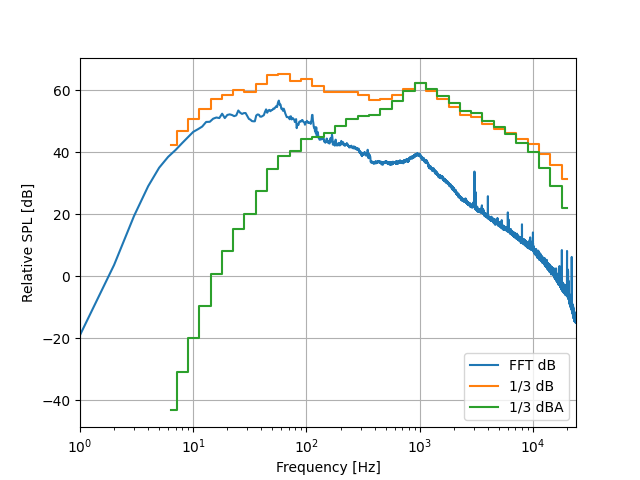
\includegraphics[width=75mm]{./Images/spectrum_plot_step.png}
    \caption{Power Spectrum for the FFT, Third-Octave-Bands, and the A-weighted Third-Octave-Bands using the 
    pre-recording reference for calibration}
    \label{fig:power_spectrum}
\end{figure}



\section{Discussion}
\subsection{Recording Site}
% construction site activity + weather

\subsection{Clipping}
% 1 event of clipping due to incredibly loud motorcycle

\subsection{Recorder}
% Gain Knobs

\subsection{Post-Processing}
% length of signal -> RAM
% scaling with 1/N caused by FFT

\section{Conclusion}

\section{References}

\end{document}

